%\documentclass[handout]{beamer}
\documentclass[t,french]{beamer}
\usepackage{babel}
\usepackage[latin1]{inputenc}
\usepackage{graphicx} %for jpg files
\usepackage{beamerthemesplit} % new 
\usetheme[compress]{Berlin}
\usecolortheme{beaver}
\usepackage{tikz}%tikz figures
\usetikzlibrary{shapes}
\usepackage{pgffor}% http://ctan.org/pkg/pgffor
\usepackage{multirow}
\usepackage{ifthen}
\usepackage{subfigure} %spacing for table of contents
%\usepackage{multimedia} %videos inside frame
\usepackage{boolexpr}
\usepackage{movie15}
%\usepackage{bbold}
\usepackage{amsmath}
\usepackage{amsfonts}
\usepackage{amssymb}

\graphicspath{{images/}}

\def\R{ \ensuremath{\mathcal{R}} }
\def\C{ \ensuremath{\mathcal{C}} }
\def\SV{ \ensuremath{\mathcal{SV}} }

\setbeamercolor{alerted text}{fg=orange}
\setbeamercolor{background canvas}{bg=white}
\setbeamercolor{block body alerted}{bg=normal text.bg!90!black}
\setbeamercolor{block body}{bg=normal text.bg!90!black}
\setbeamercolor{block body example}{bg=normal text.bg!90!black}
\setbeamercolor{block title}{bg=blue}
\setbeamercolor{fine separation line}{}
\setbeamercolor{frametitle}{fg=black,bg=gray!30}
\setbeamercolor{item projected}{fg=black}
\setbeamercolor{normal text}{bg=black,fg=black}
\setbeamercolor{palette sidebar primary}{use=normal text,fg=normal text.fg}
\setbeamercolor{palette sidebar quaternary}{use=structure,fg=structure.fg}
\setbeamercolor{palette sidebar secondary}{use=structure,fg=structure.fg}
\setbeamercolor{palette sidebar tertiary}{use=normal text,fg=normal text.fg}
\setbeamercolor{section in sidebar}{fg=black}
\setbeamercolor{section in sidebar shaded}{fg= grey}
\setbeamercolor{separation line}{}
\setbeamercolor{sidebar}{bg=red}
\setbeamercolor{sidebar}{parent=palette primary}
\setbeamercolor{structure}{bg=black, fg=red}
\setbeamercolor{subsection in sidebar}{fg=black}
\setbeamercolor{subsection in sidebar shaded}{fg=grey}
\setbeamercolor{title}{fg=black!100,bg=gray!30}
\setbeamercolor{titlelike}{fg=brown}

%several template parameters
\setbeamertemplate{frametitle}[default][center]
\setbeamertemplate{blocks}[rounded][shadow=true]
%\beamertemplateshadingbackground{white!20}{black!20}
\setbeamertemplate{background canvas}[vertical shading][bottom=white,top=white!25]
\setbeamertemplate{sidebar canvas left}[horizontal shading][left=white!40!black,right=black]
\setbeamercolor{footline in sidebar}{fg=black}%[page number]
%\setbeamertemplate{footline}[frame number]
%suppress navigational bar
\beamertemplatenavigationsymbolsempty
%experimental stuff
\setbeamertemplate{title page}[default][rounded=true,shadow=true]


% Images
\pgfdeclareimage[width=10cm]{ROSEquation}{./images/ros_equation_2}
\pgfdeclareimage[width=10cm]{gazebo}{./images/gazebo_horz_cmyk_pos.jpg}
\pgfdeclareimage[width=10cm]{opencv}{./images/opencv_logo.png}
\pgfdeclareimage[width=10cm]{pcl}{./images/pointcloudlibrary_horz_large_pos.jpg}
\pgfdeclareimage[width=10cm]{moveit}{./images/moveit-logo.png}

% Tikz libraries
\usetikzlibrary{shadows}
\usetikzlibrary{automata}
\usetikzlibrary{arrows}

% For arrows
\definecolor{darkblue}{rgb}{0.2,0.2,0.6}
\definecolor{darkred}{rgb}{0.6,0.1,0.1}
\definecolor{darkgreen}{rgb}{0.2,0.6,0.2}

\def\arrowt{
  (0.1,0.5) -- (0.0,1) -- (6.0,1.0) [rounded corners=0.5] --
  (6.0,1.5) [rounded corners=1] -- (7.0,0.5) [rounded corners=0.5] --
  (6.0,-0.5) [sharp corners] -- (6.0,0.0) -- (0.0,0.0)
  [rounded corners=1] -- (0.1,0.5) -- cycle
}

\def\arrowd{
  (10.75:1.1) -- (6.5:1) arc (6.25:120:1) [rounded corners=0.5] --
  (120:0.9) [rounded corners=1] -- (130:1.1) [rounded corners=0.5] --
  (120:1.3) [sharp corners] -- (120:1.2) arc (120:5.25:1.2)
  [rounded corners=1] -- (10.75:1.1) -- (6.5:1) -- cycle
}

\def\arrow{
  (10.75:1.1) -- (6.5:1) arc (6.25:90:1) [rounded corners=0.5] --
  (90:0.9) [rounded corners=1] -- (100:1.1) [rounded corners=0.5] --
  (90:1.3) [sharp corners] -- (90:1.2) arc (90:5.25:1.2)
  [rounded corners=1] -- (10.75:1.1) -- (6.5:1) -- cycle
}

\def\arrowtd{
  (-10.75:1.1) -- (-6.5:1) arc (-6.25:-170:1) [rounded corners=0.5] --
  (-170:0.9) [rounded corners=1] -- (-180:1.1) [rounded corners=0.5] --
  (-170:1.3) [sharp corners] -- (-170:1.2) arc (-170:-5.25:1.2)
  [rounded corners=1] -- (-10.75:1.1) -- (-6.5:1) -- cycle
}

\tikzset{
  ashadow/.style={opacity=.25, shadow xshift=0.07, shadow yshift=-0.07},
}


\def\arrows[#1]{         
  \begin{scope}[scale=#1]
    \draw[color=darkred, %
    drop shadow={ashadow, color=red!60!black}] \arrow;

    %\draw[color=darkgreen, bottom color=green!90!black, top color=green!60, %
    %drop shadow={ashadow, color=green!60!black}] [rotate=120] \arrow;

    %\draw[color=darkblue, right color=blue, left color=blue!60, %
    %drop shadow={ashadow, color=blue!60!black}] [rotate=240] \arrow;

    % to hide the green shadow

  \end{scope}
}

\include{commands}

\setlength{\unitlength}{\textwidth}  % measure in textwidths
\begin{document}

\title{Introduction ROS}

\author{Olivier Stasse \\ LAAS-CNRS, Toulouse, France}
%-- \insertframenumber/\inserttotalframenumber}

\date{20-21/05/2014} 

\AtBeginSection[]
{
  \begin{frame}
    \frametitle{Table des mati�res}
    \tableofcontents[currentsection,
      hideothersubsections]
  \end{frame}
}
%%%%%%%%%%%%%%%%%%%%%%%%%%%%%%%%%%%%%%%%%%%%%%%%%%%%%%%%%%%%%%%%%%%%%%%%%%%%%%%
{
  \usebackgroundtemplate{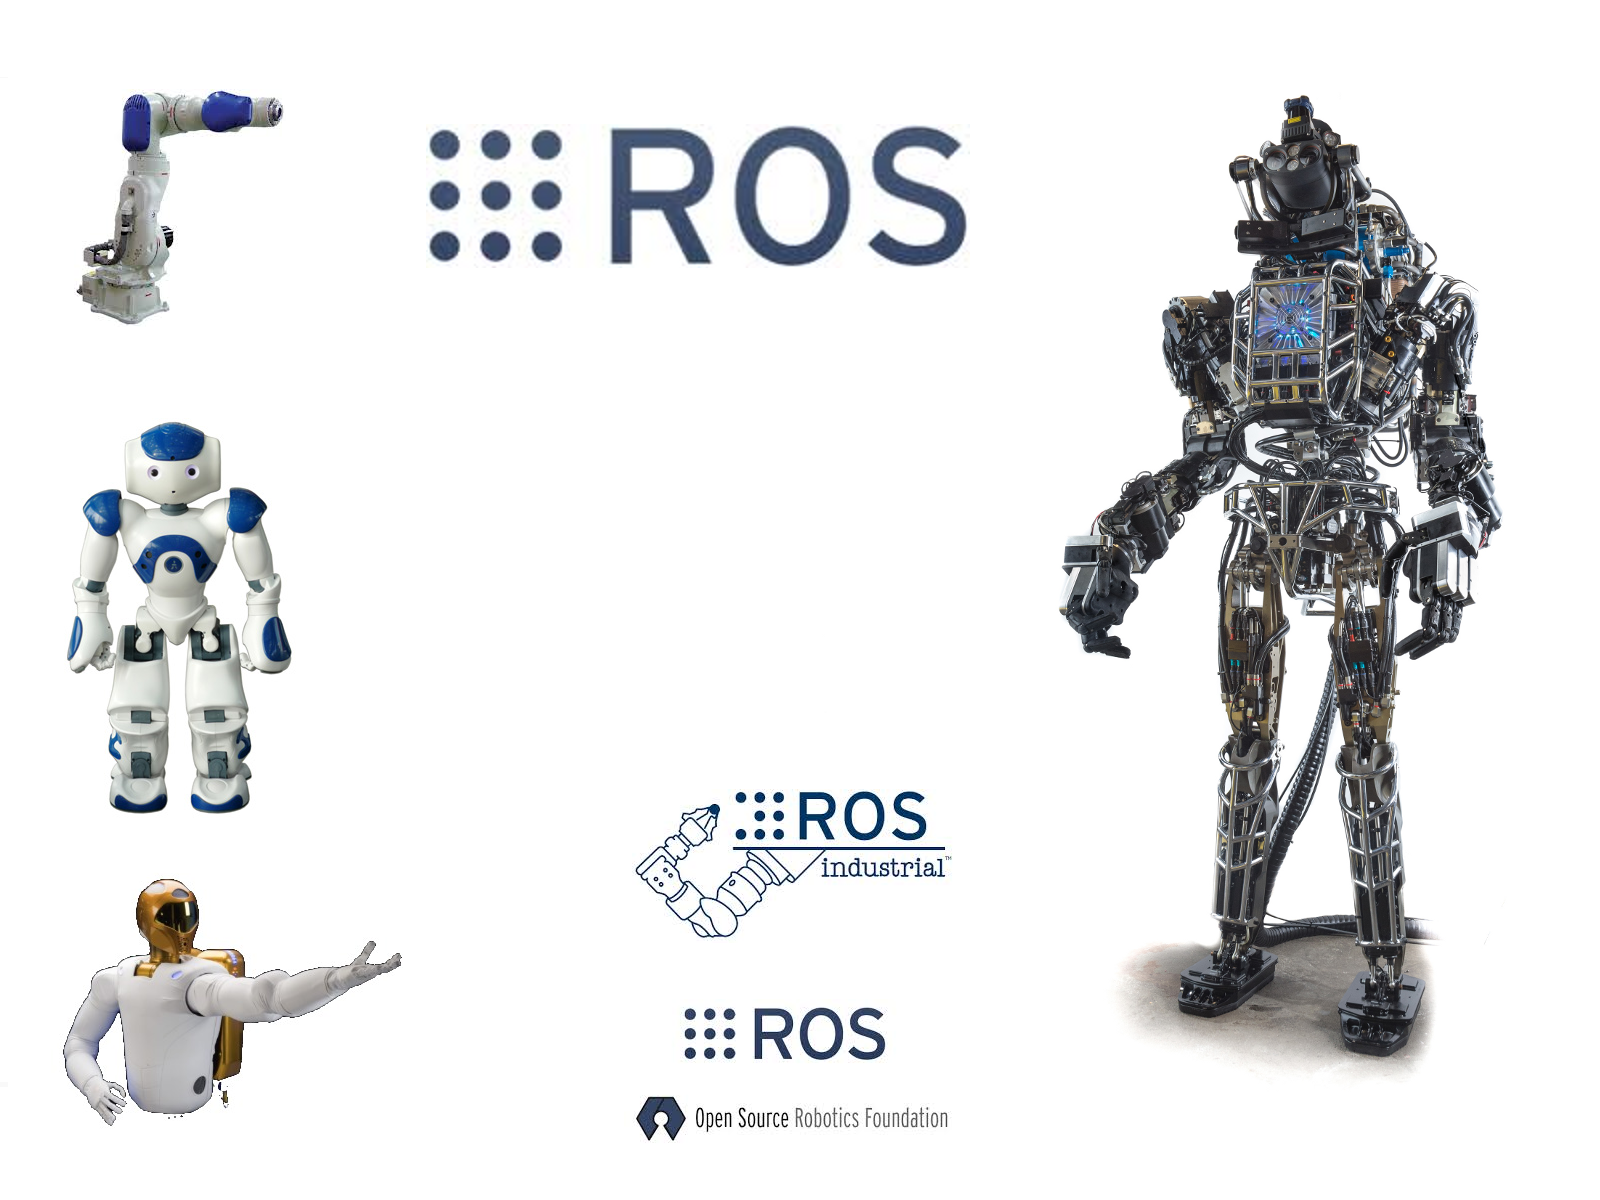
\includegraphics[width=1.0\paperwidth]{images/background-title-3.png}}
  \begin{frame}[plain]
    %\tikzstyle{stringbox}=[rectangle,color=black,fill=blue!10,text=black,draw,text opacity=0.4,align=flush center]
    \begin{tikzpicture}[remember picture, overlay]
       \node [yshift=1.8cm, xshift=-1cm, text width=4cm] (title) at (current page.center) 
            { Introduction � ROS \\
              Formation AIP};
       \node [xshift=-3.1cm,yshift=0.5cm,
              fill=white!10,fill opacity=0.7,right,text width=3cm]
             (author) at (current page.center) [scale=0.7]
            {
              Olivier STASSE, \\
              CR-1, CNRS, \\
              Gepetto, \\
              LAAS CNRS
            }; 
       \node [xshift=-3.1cm,yshift=-0.8cm,
              fill=white!10,fill opacity=0.7,
              right,text width=3cm]
        (author) 
        at (current page.center)
            {
              AIP, Toulouse\\
              $20-21$ Mai
              2014
            }; 
    \end{tikzpicture}
  \end{frame}
}
\begin{frame}
  \frametitle{Table des mati�res}
  \tableofcontents
\end{frame}
\section{Panorama}
%%%%%%%%%%%%%%%%%%%%%%%%%%%%%%%%%%%%%%%%%%%%%%%%%%%%%%%%%%%%%%%%%%%%%%%%%%%%%%%
%
\begin{frame}
\frametitle{Motivations}
\begin{block}{Passage � l'�chelle}
La communaut� robotique doit \textit{collaborer} pour cr�er des syst�mes robotiques
de qualit� � l'exemple de l'informatique et la physique. \\
ROS est l'outil qui a permis ce passage. 
\end{block}

\begin{tikzpicture}[remember picture, overlay]
  %\draw[help lines] (0,-3) grid (10,0);
  \pgfputat{\pgfxy(0.0,-2.5)}{\pgfbox[left,base]{\pgfuseimage{ROSEquation}}};
  \node[xshift=3cm,yshift=-2.5cm]{Plomberie};
  \node[xshift=5cm,yshift=-2.5cm]{Outils};
  \node[xshift=7.15cm,yshift=-2.5cm]{Capacit�s};
  \node[xshift=9.21cm,yshift=-2.5cm]{Ecosyst�me};
  %\node at (0,0) {(0,0)};	
\end{tikzpicture}
\end{frame}
%%%%%%%%%%%%%%%%%%%%%%%%%%%%%%%%%%%%%%%%%%%%%%%%%%%%%%%%%%%%%%%%%%%%%%%%%%%%%%%%%
\begin{frame}
  \frametitle{Motivations - Application robotique \only<2>{- Outils}\only<3>{distribu�e}
  }
  
  \motivationpicture
  \motivationgraph
  \visible<1-2>{\logicalrelationship}
  \visible<2>{
    \implementationgraph
  }
  \visible<3>{
    \deploymentgraph
    \softwarerelationship
  }
\end{frame}
%
%%%%%%%%%%%%%%%%%%%%%%%%%%%%%%%%%%%%%%%%%%%%%%%%%%%%%%%%%%%%%%%%%%%%%%%%%%%%%%%%%
\begin{frame}
  \frametitle{Motivations - Plomberie}
  \begin{block}{Middleware}
    \begin{itemize}     
      \item Publication/souscription � la transmission de messages anonymes (Message Passing)
      \item Enregistrer et rejouer des messages
      \item Requ�tes/r�ponses � des remote procedure calls
      \item Syst�me de param�tres distribu�s
    \end{itemize}
  \end{block}
  %
  %\begin{tikzpicture}
  %  \draw[help lines] (0,-3) grid (10,0);
  %  \node at (0,0) {(0,0)};	
  %\end{tikzpicture}
\end{frame}
%%%%%%%%%%%%%%%%%%%%%%%%%%%%%%%%%%%%%%%%%%%%%%%%%%%%%%%%%%%%%%%%%%%%%%%%%%%%%%%%%
\begin{frame}
\frametitle{ROS: Bref historique}
 \vskip -0.25cm
 \begin{tabular}{|p{3cm}|p{7.5cm}|} \hline 
   2008 & D�marrage de ROS par Willow Garage \\ 
   2010 - Janvier & ROS 1.0 \\
   2010 - Mars & Box Turtle \\
   2010 - Aout & C Turtle \\
   2011 - Mars &  Diamondback \\
   2011 - Aout & Electric Emys \\
   2012 - Avril & Fuerte \\
   2012 - D�cembre & Groovy Galapagos\\
   2013 - F�vrier & Open Source Robotics Fundation poursuit la gestion de ROS \\
   2013 - Aout & Willow Garage est absorb� par Suitable Technologies \\
   2013 - Aout & PR-2 is supported now by Clearpath Robotics\\
   2013 - Septembre& Hydro Medusa \\ \hline
 \end{tabular}
\end{frame}
%%%%%%%%%%%%%%%%%%%%%%%%%%%%%%%%%%%%%%%%%%%%%%%%%%%%%%%%%%%%%%%%%%%%%%%%%%%%%%%%%
\begin{frame}
  \frametitle{Motivations - Outils}
  \begin{itemize}
    \item[rviz] Visualisateur graphique 3D.
    \item[rosbag] Enregistrement et visualisation des donn�es.
    \item[rxplot] Affichage en ligne.
    \item[rxgraph] Visualisation du syst�me.
    \item[catkin] Syst�me de compilation et de gestion de paquets.
  \end{itemize}
\end{frame}
%%%%%%%%%%%%%%%%%%%%%%%%%%%%%%%%%%%%%%%%%%%%%%%%%%%%%%%%%%%%%%%%%%%%%%%%%%%%%%%%%
\begin{frame}
  \frametitle{Motivations - Ecosyst�me}
  \vskip 0.25cm
  \begin{itemize}
    \item D�finitions de messages standards pour les robots
    \item Librairie pour la g�om�trie des robots
    \item Language de description des robots
    \item Remote Procedure Calls pr�emptable
    \item Diagnostiques
    \item Estimation de pose
    \item Localisation
    \item Cartographie
    \item Navigation
  \end{itemize}
\end{frame}
%%%%%%%%%%%%%%%%%%%%%%%%%%%%%%%%%%%%%%%%%%%%%%%%%%%%%%%%%%%%%%%%%%%%%%%%%%%%%%%%%
\begin{frame}
  \frametitle{Motivations - Ecosyst�me}
  \begin{itemize}
    \item Syst�mes d'exploitation
    \item Robots
    \item 
  \end{itemize}
\end{frame}
%%%%%%%%%%%%%%%%%%%%%%%%%%%%%%%%%%%%%%%%%%%%%%%%%%%%%%%%%%%%%%%%%%%%%%%%%%%%%%%%%
\section{Communications ROS}
%%%%%%%%%%%%%%%%%%%%%%%%%%%%%%%%%%%%%%%%%%%%%%%%%%%%%%%%%%%%%%%%%%%%%%%%%%%%%%%%%
\begin{frame}
  \frametitle{}
\end{frame}
%%%%%%%%%%%%%%%%%%%%%%%%%%%%%%%%%%%%%%%%%%%%%%%%%%%%%%%%%%%%%%%%%%%%%%%%%%%%%%%%%
\section{Organisation des programmes sous ROS}
%%%%%%%%%%%%%%%%%%%%%%%%%%%%%%%%%%%%%%%%%%%%%%%%%%%%%%%%%%%%%%%%%%%%%%%%%%%%%%%%%

%%%%%%%%%%%%%%%%%%%%%%%%%%%%%%%%%%%%%%%%%%%%%%%%%%%%%%%%%%%%%%%%%%%%%%%%%%%%%%%%%
\section{Programmer avec ROS}
%%%%%%%%%%%%%%%%%%%%%%%%%%%%%%%%%%%%%%%%%%%%%%%%%%%%%%%%%%%%%%%%%%%%%%%%%%%%%%%%%

%%%%%%%%%%%%%%%%%%%%%%%%%%%%%%%%%%%%%%%%%%%%%%%%%%%%%%%%%%%%%%%%%%%%%%%%%%%%%%%%%
\section{La librairie TF}
%%%%%%%%%%%%%%%%%%%%%%%%%%%%%%%%%%%%%%%%%%%%%%%%%%%%%%%%%%%%%%%%%%%%%%%%%%%%%%%%%

%%%%%%%%%%%%%%%%%%%%%%%%%%%%%%%%%%%%%%%%%%%%%%%%%%%%%%%%%%%%%%%%%%%%%%%%%%%%%%%%%
\section{Programmer un noeud ROS}
%%%%%%%%%%%%%%%%%%%%%%%%%%%%%%%%%%%%%%%%%%%%%%%%%%%%%%%%%%%%%%%%%%%%%%%%%%%%%%%%%

%%%%%%%%%%%%%%%%%%%%%%%%%%%%%%%%%%%%%%%%%%%%%%%%%%%%%%%%%%%%%%%%%%%%%%%%%%%%%%%%%
\begin{frame}{Conclusions}
\end{frame}
%%%%%%%%%%%%%%%%%%%%%%%%%%%%%%%%%%%%%%%%%%%%%%%%%%%%%%%%%%%%%%%%%%%%%%%%%%%%%%%%%
%

\end{document}

